\tikzset{every picture/.style={line width=0.75pt}} %set default line width to 0.75pt        

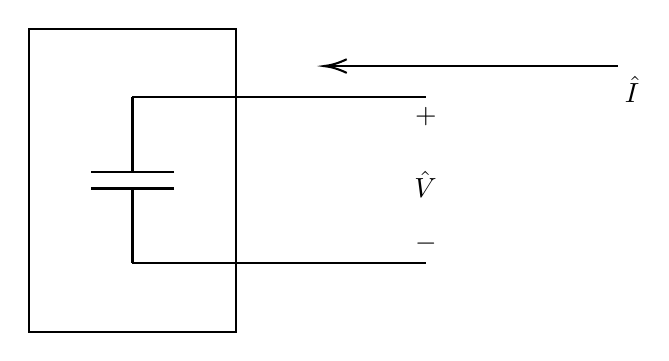
\begin{tikzpicture}[x=0.75pt,y=0.75pt,yscale=-1,xscale=1]
%uncomment if require: \path (0,300); %set diagram left start at 0, and has height of 300

%Shape: Rectangle [id:dp6052217164752943] 
\draw   (139,64) -- (239,64) -- (239,210) -- (139,210) -- cycle ;
%Shape: Capacitor [id:dp8313198965554979] 
\draw   (189,97) -- (189,133) (209,141) -- (169,141) (209,133) -- (169,133) (189,141) -- (189,177) ;
%Straight Lines [id:da9264456177024911] 
\draw    (189,97) -- (330.42,97) ;
%Straight Lines [id:da07843275164062369] 
\draw    (189,177) -- (330.42,177) ;
%Straight Lines [id:da17167344062070922] 
\draw    (422.71,82) -- (283.29,82) ;
\draw [shift={(281.29,82)}, rotate = 360] [color={rgb, 255:red, 0; green, 0; blue, 0 }  ][line width=0.75]    (10.93,-3.29) .. controls (6.95,-1.4) and (3.31,-0.3) .. (0,0) .. controls (3.31,0.3) and (6.95,1.4) .. (10.93,3.29)   ;

% Text Node
\draw (330.42,100.4) node [anchor=north] [inner sep=0.75pt]    {$+$};
% Text Node
\draw (330.42,173.6) node [anchor=south] [inner sep=0.75pt]    {$-$};
% Text Node
\draw (330.13,131.4) node [anchor=north] [inner sep=0.75pt]    {$\hat{V}$};
% Text Node
\draw (424.71,85.4) node [anchor=north west][inner sep=0.75pt]    {$\hat{I}$};


\end{tikzpicture}
